\chapter{Methodology}\label{sec:meth}
This dissertation will evaluate Rust through the compared performance of  kernels, using the test data to find any weaknesses in the Rust or original implementation. The experience of learning and programming in Rust will also be documented.

I am going to use Kernels rather than mini-apps because mini apps often focus on a particular scientific domain, whilst performing the same sort of calculations. For example, a meteorological mini-app and a fluid dynamics mini-app might both use the Jacobi method~\cite{muller2014, schippers1982}, but only differ in their input and preconditioning of data.
Through only attempting to port the core part of a program, this dissertation will be able to examine a breadth of use case scenarios, hopefully without losing any of the depth of examining mini-apps.

I will also evaluate the ease with which I am able to port a kernel into Rust. These observations will provide insight into what it is like to program in Rust, and if its strict memory model and functional idioms help or hinder translation from the imperative languages which the ported programs are written in. This qualitative, partly experiential information will hopefully provide an insight into the actual practicalities of programming in Rust. For Rust to be fully accepted by the HPC community, it is necessary that the program fulfils the functional requirements of speed and scaling, alongside non functional requirements, of usability and user experience. The first factor provides a reason for using Rust programs in HPC, the second provides an impetus for learning how to write those programs.

I will use reference implementations of the kernels that have already been written by other people rather than writing my own. I will do this for two reason. Firstly, a fairer comparison between Rust and C or C++ can be made if I do not write the original implementation myself, so that my lack of knowledge in one of the programs makes it perform worse. Secondly, by selecting reference implementations that have already been written, I can save time and not write them myself, allowing me a deeper investigation of the Rust implementations.

\section{Kernel Selection}
So that a breadth of usage scenarios were examined, three kernels were selected based on their conformity to a pre-defined set of criteria. The criteria were proposed during my project preparation, and have been finalised below.
\begin{itemize}
  \item \textbf{The part of the program responsible for more than two thirds of the processing time should not be more than 1500 lines.} To ensure that I fully implemented three ports of existing kernels, it was necessary to limit the size of the kernels that could be considered. Whilst it reduced the field of possible kernels, it helpfully excluded any overly complex mini-apps.

  \item \textbf{The program must target the CPU}Programs which target the GPU rather than the CPU will not be considered, as the current implementations for Rust to target GPUs involve calling out to existing GPU APIs. Therefore, any analysis of a Rust program targeting a GPU would largely be an analysis of the GPU API itself.

  \item \textbf{The program must use shared memory parallelism and target the CPU.} Rust's (supposed) zero cost memory safety features are its differentiating factor. The best way to test the true cost of Rust's memory safety features would be through shared memory parallelism, where a poor implementation of memory management will make itself evident through poor performance.
  
  \item \textbf{The program run time should reasonably decrease as the number of threads increases, at least until the number of threads reaches 32.} It is important that any kernel considered is capable of scaling to the high core counts normally seen in HPC.I will be running the kernels on Cirrus, which supports 36 real threads.

  \item \textbf{The program operate on data greater than the CPU's L3 Cache} so that I can be sure that the kernel is representative of working on large data sets. Cirrus has an L3 cache of 45MiB. As each node has 256GB of RAM, a central constraint when working with large data sets is the speed with which data is loaded into the cache. 

  \item \textbf{The program must be written in C or C++.} This restriction allows us to choose work which is more representative of HPC programs that actually run on HPC systems, rather than python programs which call out to pre-compiled libraries. Unlike Fortran, C and C++ use array indexing and layout conventions similar to Rust, which will make porting programs from them easier.

  \item \textbf{The program must use OpenMP.} This is a typical approach for shared memory parallelism in HPC\@. Use of a library to do the parallel processing also further standardises the candidate programs, which will lead to a deeper understanding of the kernel's performance factors.
\end{itemize}

I used these selection criteria to compile a long list of potential kernels to port to Rust. From this long list, I selected BabelStream, sparse matrix-vector multiplication and K-means clustering. An example of a kernel I rejected is given in Section~\ref{sec:pipe}.

\subsection{BabelStream}

BabelStream is a memory bench marking tool which was developed by researchers at the university of Bristol~\cite{Babel2018}. BabelStream was written to primarily target GPUs, but it is able to target CPUs too~\cite{BabelStream}.
It is written in C++, supports OpenMP and allows one to set the problem size when executing the program, so I can be sure the kernel's data exceeds the size of L3 cache. My initial tests found the kernel to scale well, and although the program as a whole is quite large, when one ignores the parallel technologies excluded by my selection criteria, the amount of code which needs to be ported to Rust falls well within my bounds. I found BabelStream easy to install and run.

BabelStream performs simple operations on three arrays of either 32 or 64 bit floating point numbers, \texttt{a}, \texttt{b} and \texttt{c}. The values of \texttt{a} are set to 0.1, \texttt{b}'s to 0.2, and \texttt{c}'s to 0.0. Stream performs five operations \texttt{n} times on the arrays, where \texttt{n} is a specified command line argument. The operations are listed below:
\begin{itemize}
  \item \textbf{Copy:} Data is copied from the array \texttt{a} into array \texttt{c}
  \item \textbf{Multiply:} Data in \texttt{c} is multiplied by a scalar and stored in \texttt{b}
  \item \textbf{Add:} The values in \texttt{a} and \texttt{b} are added together and stored in \texttt{c}
  \item \textbf{Triad:} The program then multiplies the new values in \texttt{c} by the same scalar value, adds it to \texttt{b} and stores the value in \texttt{a}
  \item \textbf{Dot:} The dot product is performed on arrays \texttt{a} and \texttt{b}. This is when every nth element of \texttt{a} is multiplied by the nth element of \texttt{b}, and summed.
\end{itemize}
The resulting values in the arrays are then compared against separately calculated reference values, and examined to see if their average error is greater than that number type's epsilon value.

BabelStream's operations are `\textit{memory bandwidth bound}'~\cite{BabelStream}, because they are computationally simple. Therefore, when implemented through different technologies, BabelStream provides an insight into the memory bandwidth of that technology and hardware, and gives an indication of how the design choices of that technology influences its performance.

\subsection{Sparse Matrix Vector Multiplication}

The Sparse Matrix Vector Multiplication (SpMV) Kernel~\cite{ParResSparse} forms part of the Parallel Research Kernels suite, developed by the Parallel Research Tools group. SpMV is a common HPC operation, used to solve a broad range of scientific problems~\cite{Sedaghati:2015, spMVGPU, DBLP:journals}.

The kernel is mostly one file, sparse.c, which in total is 353 lines of code. The implementation is in C and OpenMP, and my tests found it to scale to a thread count of 36. As with BabelStream, the program allows one to set problem size through command line arguments, allowing me to ensure the program operated on data greater than the CPU's L3 cache.

The program represents its sparse matrix through the compressed sparse row (CSR) format \todo{diagram?}. This format uses key information about the matrix to avoid storing all of the sparse matrix's redundant zeros in the computer's memory. The information used to do this are the number of rows and columns the matrix has, and the number of non zero values which exist in the matrix. These three values are used to build three vectors, one holding all the non zero values of the matrix, another vector of the same length holding the column indexes for all of those values, in order, and lastly a smaller vector which holds the index at which a particular row starts.

For example, if I wanted the element at 24,32 within the vector, I would look in the 24\textsuperscript{th} element of the row start vector, which would give us the y index of the element. If this did not match the y index I was looking for, in this case 32, I would then look at the next element until I found it. Once I have found the element, I can get the value from the value vector using the index constructed by adding the 24\textsuperscript{th} element of the row start vector, added to however many times I needed to look at the next value to before I found the appropriate y index.

The particular implementation of SpMV which I am porting to Rust uses a user defined grid size, over which a user defined periodic stencil is applied to find the number of non zero entries. The implementation parallelises its initialisation and the actual multiplication of the values using simple \texttt{\#pragma omp parallel} statements.

This kernel will hopefully provide a realistic idea of how well Rust can perform one of the most common HPC operations.

\subsection{K-means clustering}

K-means clustering is a `process for partitioning an $N$-dimensional population into $K$ sets'~\cite{macqueen1967}, where the number of sets is less than $N$, and each set is clustered around a local mean. 
K-means clustering finds many uses in HPC, particularly in weather forcasting~\cite{DBLP:journals/corr/ChakrabortyND14a} and astrophysics~\cite{ordovas2014fast}. It has become so ubiquitous throughout HPC that implementations of it are already used to evaluate software and hardware~\cite{Yang2014}.

My reference implementation for this code comes from a Havard PhD candidate's undergraduate CS205 project~\cite{CS205}. It is written in C and uses OPENMP, and is less than 200 lines long. The data processed by the program can be generated by a script, allowing me to work on an arbitrary amount of data. The kernel is written so that all processing is done by the CPU\@. It is of particular interest that the kernel reads its data from a NetCDF file, which is common in HPC\@. The code is well documented and concise.

After the kernel has read in the program data, it performs the clustering process. The calculated clusters are held in the two dimensional vectors, \texttt{old\_cluster\_centres} and \texttt{new\_cluster\_centres}. The indexes at which values are stored in these cluster vectors correspond to the indexes at which the population is stored in the vector \texttt{x}. The population data is loaded into \texttt{x} from the NetCDF file.

First the \texttt{old\_cluster\_centres} array is filled with random data, and then the program begins its central processing loop.

\begin{itemize}
  \item \textbf{Expectation:} Assign population points to their nearest cluster centre, by looping over every member of the population, and finding the minimum distance between that point all the cluster centres. This is the stage which is parallelised.
  \item \textbf{Maximisation:} Next, the cluster centres are set to the mean, which is calculated in two steps.
  \begin{itemize}
    \item \textbf{1:} The size of the cluster is calculated by looping over every point and finding its cluster centre, and then incriminating that cluster centres population count. The sum of the points in that cluster is also calculated and stored in the \texttt{new\_cluster\_centres} array.
   \item \textbf{2:} The sum of the cluster is divided by the size of it, and stored in to the \texttt{old\_cluster\_centres} for use on the next iteration of the loop.
   \end{itemize}
\end{itemize}
This loop continues until it reaches a pre-defined maximum iteration value, or the sum of the minimum distance values becomes less than a certain tolerance value. The program then writes data back out to the NetCDF file it read the data from originally.

I found this program quite difficult to install and run due to the NetCDF dependency. My first attempt to install NetCDF through the script included in the repository ended with me unable to boot into my laptop. Subsequent attempts to install NetCDF through package managers were also not successful, although they were less damaging to my system. To compile the kernel on Cirrus I had to make sure I had selected the correct combination of NetCDF and HDF5 library versions, mostly through trial and error. However, once I had accomplished this task, compiling the program itself was easy. The kernel then showed itself to be able to scale well enough for the interests of this project.

\subsection{Pipeline}\label{sec:pipe}
The group of parallel research kernels which included SpMV also included a pipeline kernel. The kernel perfroms a relaxation over an array, where each thread became ran its own part of the pipeline. This kernel was written in C and OpenMP, and was only 328 lines long. It targeted the CPU and met all the necessary criteria, except for one. As figure~\ref{fig:pipe} shows, the kernel was unable to scale to the same extent as the other selected kernels, and was therefore rejected.

\begin{figure}[h]
\centering
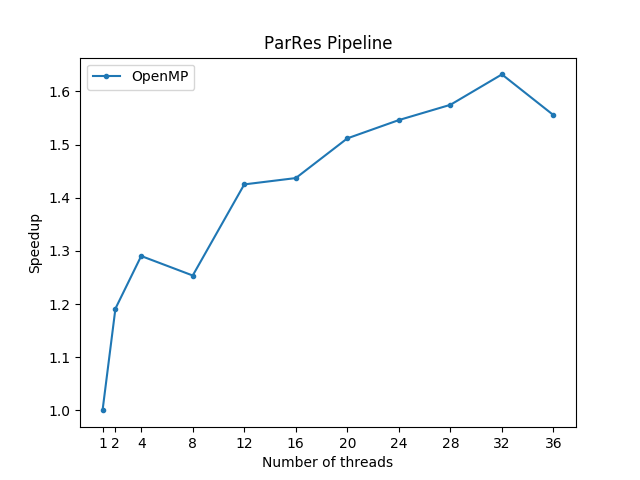
\includegraphics[width=.9\linewidth]{figs/pipe/pipe.png}
\caption[Pipeline --- Speedup]{Pipeline --- Speedup against number of threads. This graph shows that the pipeline kernel was unable to achieve even speedup of a factor of 2, even when given multiple threads.}\label{fig:pipe}
\end{figure}

\section{Implementation Methodology}
I will attempt to write Rust in an idiomatic style. This should result in Rust programs that are as representative of how actual Rust is written, as possible. Idiomatic Rust tends to chain function calls and use pattern matching to achieve more succinct code.

My implementation will attempt to be as faithful to the original implementation as possible. Therefore, if there are any improvements which can be made to the structure of the code, such as abstracting repeated code into methods, I will not make them. Lastly, if I need assistance in writing my implementation of the Rust code, I will use only freely available resources. I will, if necessary, seek assistance in Rust programming communities on the internet.


\section{Experimentation}
All experiments were run on a single node of Cirrus, an EPCC HPC Cluster. No other users had access to that node whilst experiments were being run. Each node on Cirrus has 36 cores, spread across two 18 core Intel Xeon E5-2695 processors. Each processor shares a 45MiB L3 cache between its 18 cores, with smaller L1 and L2 caches for each individual core.Each processor belongs to a separate NUMA region, leading to increased latency when retrieving data from the other NUMA region~\cite{CirrusHardware}.

Both versions of each Kernel were run for 100 iterations, and the average speed was taken. Experiments were submitted to cirrus through the use of Portable Batch Script (PBS) files, which returned program output to timestamped files. A sample PBS submission file can be found in Appendix~\ref{app:launch}.

The BabelStream experiments were run on vectors of size of 1GB, leading to a total data size of 3GB\@. Each vector was filled with $1.25\times10^8$ 64-bit floating point numbers. Experiments were run multiple times with varying chunk sizes. Chunk sizes here refers to the amount of data a thread works on, in a given iteration. Varying chunk size gave greater insight into the inner workings of the Rayon library, and see the cost of context switching for threads.

For the sparse matrix vector multiplication kernel, the vectors \texttt{col\_index} and \texttt{matrix} were given a size of 8.2GB, whilst the \texttt{result} and \texttt{vector} vectors had size 0.134 GB\@. The generated matrix had sparsity $3.63 \times 10^{-5}$. Such large vector sizes were used to ensure that a large amount of data passed through the system's L3 caches. Chunk size was not varied in this instance to allow for a clearer comparison between Rayon and OpenMP in the Roofline model. The command below was used to monitor the total number of FLOPs used by the different implementations of the kernel

\begin{alltt}
\footnotesize
perf stat -e r5301c7 -e r5302c7 -e r5304c7 -e r5308c7 -e r5310c7 
          -e r5320c7 \$kernel 
\end{alltt}

\texttt{perf} is a program performance monitor for linux systems which works at the system's kernel level, using hardware counters to track certain events. I request statistics on events with \texttt{stat}, and then specify each event after \texttt{-e}. Each of these events are floating point operations for doubles, at various levels of vectorisation. Lastly, I launch the kernel as normal, here shown by \texttt{\$kernel}.
I used \texttt{perf} to monitor all of the FLOPS of the program, as nearly all of the FLOPS in the program, including initialisation, are parallelised. Some FLOPS are used for timing purposes, but there are very few of these.

I will use the peak memory bandwidth recorded by the BabelStream kernel in my Roofline Model. For the peak Flop/s, I will use the theoretical figure calculated from the processor's specification. I am making this choice because the maximum calculated Flop/s is difficult to find due to a processor's vector units.

K-means used a population of size 73MB, and 16 clusters. This meant that the parallelised E-step of the calculation operated on total of 147MB of data, most of which were 32-bit floats. The rest of the data was 64 bit integers of type \texttt{usize} which were used to refer to array indexes. This size of data set exceeded the L3 cache capacity, but was unable to be raised due to instability in the generating python script.

A Roofline model of K-means clustering will not be generated, as a large portion of the kernel is not parallelised, including initialisation and both parts of the M-step. If a Roofline model were used in this case, it would not be greatly illustrative of the differences between the implementation, as much of the useful information from the data about the E-step would be lost in the noise of the rest of the processing time.

I used version 6.3.0 of GNU project C and C++ compiler, \texttt{gcc} and \texttt{g++} to compile the reference implementations of the kernels. Version 1.34.2 of the Rust compiler, \texttt{rustc} was used. Although \texttt{rustc} and the C compiler \texttt{clang} have the same LLVM backend, \texttt{clang} so that the comparison would not become about how each language's compiler best uses LLVM\@.
\section{Questionnaire}\label{sec:meth-q}
To further assess the suitability of Rust for HPC, I presented staff and students at EPCC with a questionnaire. The aim of this questionnaire was to examine how easily people with little to no experience of Rust could understand it. The more understandable a language is, the easier it is to learn, the more likely it is to be adopted. This questionnaire would provide valuable data on the usability of Rust as a language.

The questionnaire was formed of seven multiple choice questions, designed to test the participant's ability to understand Rust. Each question first presented the participant with a fragment of Rust code, and was then asked what that fragment of code did. On some questions, context specific information was given to the participant, such as on question four, which told the participant that `A vector's pop method return an optional value, or none'. The decision to give the participant this extra information was made so that they could deal with certain functionality which was not unique to Rust, but had a particular name which might be different to something they had already encountered in another language. In this case, the idea of the optional value is seen in other languages, like Haskell's Maybe type~\cite{HaskellMaybe}.

An eighth question was also given, which asked the participant how skilled they were at various programming languages.
To minimise the factors of impostor syndrome~\cite{langford1993} and the Dunning-Kruger effect~\cite{kruger1999} on this question, (which were hopefully minimal due to the anonymous nature of the questionnaire), each skill level was given concrete examples of what they corresponded to. For example, basic knowledge was the ability to `write loops, [and] conditionals', whilst advanced knowledge was the ability to `effectively use the more esoteric features of this language'. Self assessment will never be as good as independent assessment, but without the ability to ask for a large amount of time from my participants, it had to suffice.

This last question was used to generate a competency score, with different levels of reported competency receiving a different score. Basic competency in a programming language received a score of one, comprehensive two, and advanced three. The sum of all these scores became that participants competency score.

The questionnaire was left out in the lunch area at 12am. Staff and academics were notified of its presence via email at 11:30am and questionnaires were collected at 5pm. I watched the first few questionnaires be completed, but did not intervene in the process. I then returned to my desk to make sure I did not affect the data collection through my presence. As all the questionnaires were anonymous, and the people answering them all had a limited amount of time and low investment in the results, people cheating on the questionnaire was not considered a risk. 

A full copy of the questionnaire can be found in Appendix~\ref{app:quest}.
